\chapter{Implementasi dan Pengujian}
\label{chap:implementasipengujian}

Bab ini membahas tentang implementasi dan pengujian perangkat lunak berdasarkan rancangan yang sudah dibuat. Ada dua jenis pengujian yang dilakukan, yaitu pengujian fungsional, pengujian keakuratan, dan pengujian eksperimental. Bab ini juga membahas tentang lingkungan yang digunakan untuk pengujian perangkat lunak ini.

\section{Lingkungan untuk Pengujian}
\label{sec:lingkunganpengujian}

Pengujian perangkat lunak ini dilakukan di Lab Komputasi FTIS Unpar ruang 9018. Semua \textit{file} permainan yang dipakai dalam pengujian ini dapat dilihat di bab Lampiran~\ref{chap:soalsoal}. 

Ada dua jenis lingkungan untuk pengujian perangkat lunak ini, yaitu:

\begin{enumerate}
\item Lingkungan perangkat keras, yaitu lingkungandigunakan untuk pengujian perangkat lunak ini memiliki spesifikasi berikut:

\begin{table}
\centering
\captionsetup{justification=centering}
\caption[Lingkungan perangkat keras untuk pengujian perangkat lunak]{Lingkungan perangkat keras untuk pengujian perangkat lunak}
\begin{tabular}{| l | l |}
\hline
Parameter & Nilai \\
\hline \hline
\textit{Processor} & Lorem Ipsum \\
\hline
\textit{RAM (Random Access Memory)} & Lorem Ipsum \\
\hline
\textit{VGA (Video Graphics Array)} & Lorem Ipsum \\
\hline
\end{tabular}
\label{tab:lingkunganpk}
\end{table}

\item Lingkungan perangkat lunak, yaitu lingkungan yang digunakan untuk pengujian perangkat lunak ini memiliki spesifikasi berikut:

\begin{table}
\centering
\captionsetup{justification=centering}
\caption[Lingkungan perangkat lunak untuk pengujian perangkat lunak]{Lingkungan perangkat lunak untuk pengujian perangkat lunak}
\begin{tabular}{| l | l |}
\hline
Parameter & Nilai \\
\hline \hline
Sistem Operasi & Lorem Ipsum \\
\hline
Bahasa Pemrograman & Java \\
\hline
\textit{IDE (Integrated Development Environment)} & NetBeans IDE 8.2 \\
\hline
\textit{Library Java} & JDK (\textit{Java Development Kit}) 1.8 \\
\hline
\textit{JVM (Java Virtual Machine)} & Java Version 8 Update Lorem Ipsum \\
\hline
\end{tabular}
\label{tab:lingkunganpl}
\end{table}

\end{enumerate}

\section{Implementasi}
\label{sec:implementasi}

Hasil implementasi dari rancangan perangkat lunak yang sudah dibuat ini terdiri dari dua bagian, yaitu:

\begin{enumerate}
\item Kode program
\item Antarmuka perangkat lunak
\end{enumerate}

Kedua bagian tersebut akan dijelaskan lebih lanjut di bawah ini.

\subsection{Kode Program}
\label{sec:kodeprogram}

Kode program untuk perangkat lunak ini ditulis dalam bahasa pemrograman Java, berdasarkan dengan rancangan diagram kelas yang sudah dibuat, seperti dapat dilihat pada sub-bab~\ref{sec:diagramkelas}. Seluruh kode program untuk perangkat lunak ini dapat dilihat di bab Lampiran~\ref{chap:kodeprogram}.

\subsection{Antarmuka Perangkat Lunak}
\label{sec:antarmukapl}

Antarmuka untuk perangkat lunak ini dirancang berdasarkan rancangan yang sudah dibuat, seperti dapat dilihat pada sub-bab~\ref{sec:perancanganantarmuka}.

Gambar~\ref{fig:antarmukapl1} menunjukkan antarmuka perangkat lunak saat pertama kali dibuka, sebelum \textit{file} permainan dibuka. Gambar~\ref{fig:antarmukapl2} menunjukkan kotak dialog untuk memilih \textit{file} permainan yang akan dibuka. Gambar~\ref{fig:antarmukapl3} menunjukkan antarmuka perangkat lunak setelah membuka \textit{file} permainan yang dipilih. Gambar~\ref{fig:antarmukapl4} menunjukkan kotak dialog untuk mengatur nilai untuk parameter-parameter algoritma genetik. Gambar~\ref{fig:antarmukapl5} menunjukkan antarmuka perangkat lunak setelah permainan berdasarkan \textit{file} permainan yang telah dibuka diselesaikan.

\begin{figure}
\centering
\captionsetup{justification=centering}
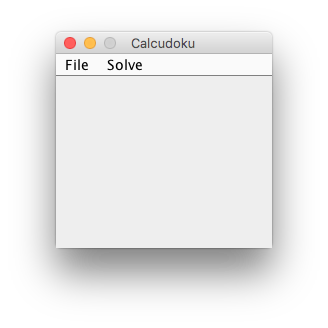
\includegraphics[scale=0.5]{Gambar/ImplementasiPengujian/Calcudoku1.png}
\caption[Antarmuka perangkat lunak saat pertama kali dibuka]{Antarmuka perangkat lunak saat pertama kali dibuka}
\label{fig:antarmukapl1}
\end{figure}

\begin{figure}
\centering
\captionsetup{justification=centering}
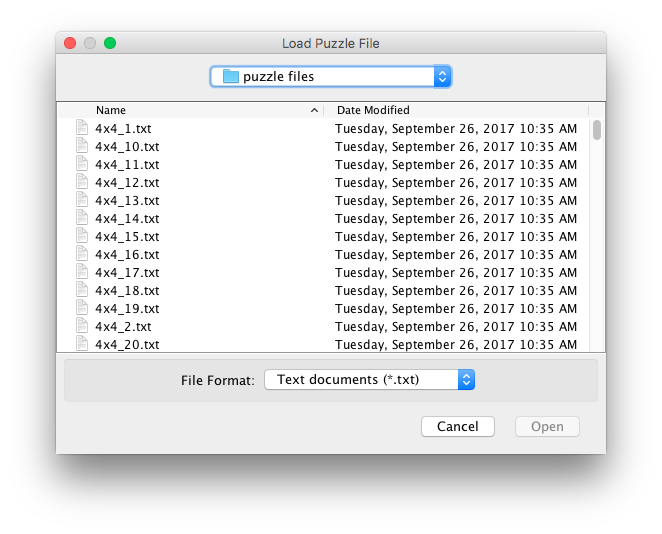
\includegraphics[scale=0.5]{Gambar/ImplementasiPengujian/FileChooser.png}
\caption[Kotak dialog untuk memilih \textit{file} permainan yang akan dibuka]{Kotak dialog untuk memilih \textit{file} permainan yang akan dibuka}
\label{fig:antarmukapl2}
\end{figure}

\begin{figure}
\centering
\captionsetup{justification=centering}
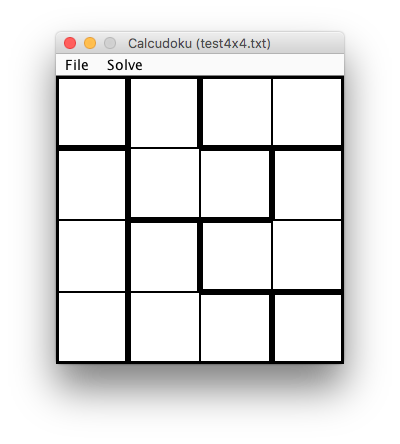
\includegraphics[scale=0.5]{Gambar/ImplementasiPengujian/Calcudoku2.png}
\caption[Antarmuka perangkat lunak sesudah membuka \textit{file} permainan yang dipilih]{Antarmuka perangkat lunak sesudah membuka \textit{file} permainan yang dipilih}
\label{fig:antarmukapl3}
\end{figure}

\begin{figure}
\centering
\captionsetup{justification=centering}
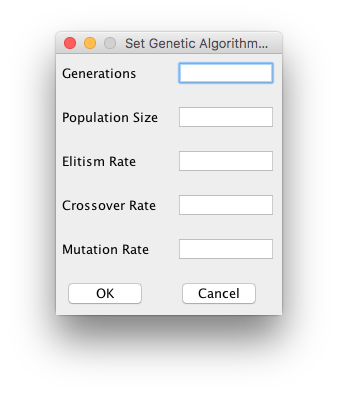
\includegraphics[scale=0.5]{Gambar/ImplementasiPengujian/SetGAParameters.png}
\caption[Kotak dialog untuk mengatur nilai dari parameter-parameter algoritma genetik]{Kotak dialog untuk mengatur nilai dari parameter-parameter algoritma genetik}
\label{fig:antarmukapl4}
\end{figure}

\begin{figure}
\centering
\captionsetup{justification=centering}
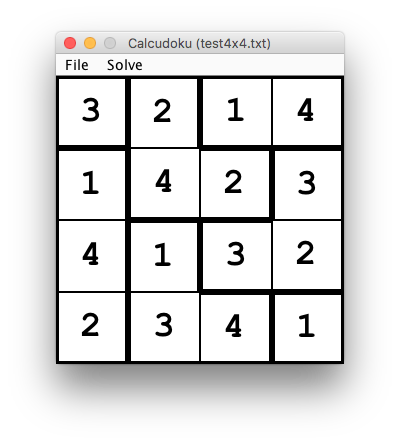
\includegraphics[scale=0.5]{Gambar/ImplementasiPengujian/Calcudoku3.png}
\caption[Antarmuka perangkat lunak setelah permainan berdasarkan \textit{file} permainan yang telah dibuka diselesaikan]{Antarmuka perangkat lunak setelah permainan berdasarkan \textit{file} permainan yang telah dibuka diselesaikan}
\label{fig:antarmukapl5}
\end{figure}

\clearpage

\section{Pengujian Fungsional}
\label{sec:pengujianfungsional}

Pengujian fungsional bertujuan untuk memastikan bahwa perangkat lunak dapat berfungsi sebagaimana mestinya. Skenario-skenario yang dilakukan dalam pengujian fungsional untuk perangkat lunak ini adalah:

\begin{enumerate}
\item Memilih menu \textit{item} "\textit{Reset Puzzle}", "\textit{Close Puzzle File}", dan "\textit{Check Puzzle}" dari menu "\textit{File}" atau menu \textit{item} "\textit{Backtracking}", "\textit{Hybrid Genetic}", dan "\textit{Set Genetic Algorithm Parameters}" dari menu "\textit{Solve}" sebelum membuka \textit{file} permainan.

Jika salah satu dari menu \textit{item} tersebut dipilih sebelum membuka \textit{file} permainan, maka pesan error "\textit{Puzzle file not loaded}" akan muncul, seperti dapat dilihat pada Gambar~\ref{fig:puzzlefilenotloaded}.

\begin{figure}
\centering
\captionsetup{justification=centering}
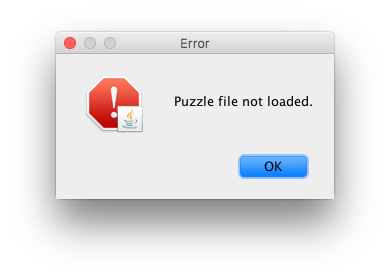
\includegraphics[scale=0.5]{Gambar/ImplementasiPengujian/PuzzleFileNotLoaded.png}
\caption[Kotak pesan error "\textit{Puzzle file not loaded}"]{Kotak pesan error "\textit{Puzzle file not loaded}"}
\label{fig:puzzlefilenotloaded}
\end{figure}

\item Membuka \textit{file} permainan

Pemain dapat membuka \textit{file} permainan pengan memilih menu \textit{item} "\textit{Load Puzzle File}" dalam menu "\textit{File}". Jika menu tersebut dipilih maka akan keluar kotak pemilihan \textit{file} permainan, seperti dapat dilihat pada Gambar~\ref{fig:filechooser}. Pilihlah sebuah \textit{file} permainan yang ingin dibuka. Tekan tombol "OK" untuk membuka \textit{file} permainan tersebut, atau tekan tombol "\textit{Cancel}" untuk membatalkan proses membuka \textit{file} permainan.

\begin{figure}
\centering
\captionsetup{justification=centering}
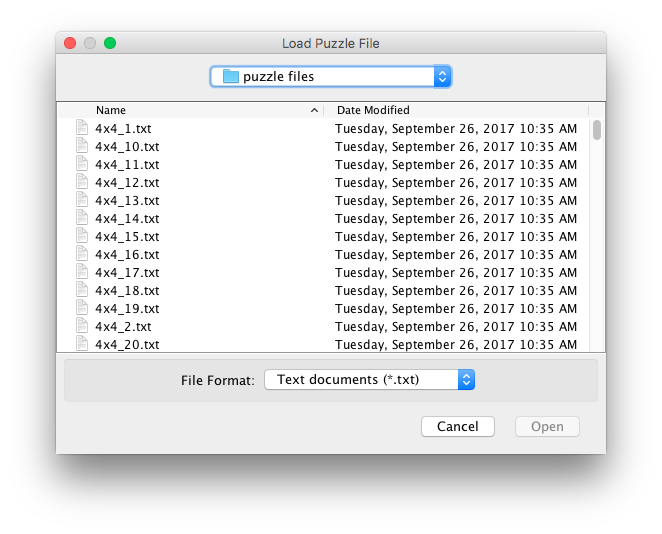
\includegraphics[scale=0.5]{Gambar/ImplementasiPengujian/FileChooser.png}
\caption[Kotak pemilihan \textit{file} permainan]{Kotak pemilihan \textit{file} permainan}
\label{fig:filechooser}
\end{figure}

Jika perangkat lunak sudah membuka sebuah \textit{file} permainan, maka akan keluar kotak dialog "\textit{Are you sure you want to load another puzzle file?}", seperti dapat dilihat pada Gambar~\ref{fig:loadpuzzlefile}. Tekan tombol "Yes" untuk membuka \textit{file} permainan tersebut, atau tekan tombol \textit{"No"} untuk membatalkan proses membuka \textit{file} permainan.

\begin{figure}
\centering
\captionsetup{justification=centering}
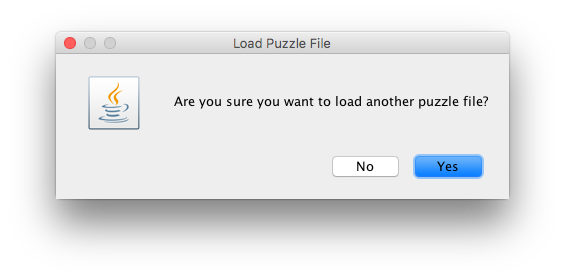
\includegraphics[scale=0.5]{Gambar/ImplementasiPengujian/LoadPuzzleFile.png}
\caption[Kotak dialog "\textit{Are you sure you want to load another puzzle file?}"]{Kotak dialog "\textit{Are you sure you want to load another puzzle file?}"}
\label{fig:loadpuzzlefile}
\end{figure}

Jika \textit{file} permainan yang dipilih berhasil dibuka, maka perangkat lunak akan menampilkan permainan berdasarkan \textit{file} yang dipilih, seperti dapat dilihat pada Gambar~\ref{fig:antarmukapl3}.

\textit{File} permainan untuk perangkat lunak ini adalah \textit{file} teks (*.txt). Format \textit{file} permainan yang valid dapat dilihat di sub-bab~\ref{sec:perancanganmasukan}.

Jika \textit{file} permainan yang dibuka tidak \textit{valid}, misalnya karena \textit{file} permainan yang dibuka bukan \textit{file} teks, atau jika \textit{file} teks yang akan dibuka formatnya tidak \textit{valid}, maka pesan error "\textit{Invalid puzzle file}" akan muncul, seperti dapat dilihat pada Gambar~\ref{fig:invalidpuzzlefile}.

\begin{figure}
\centering
\captionsetup{justification=centering}
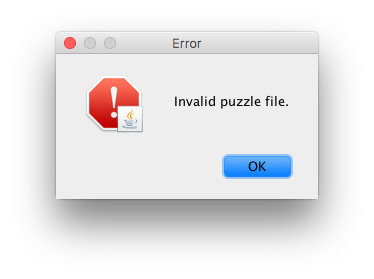
\includegraphics[scale=0.5]{Gambar/ImplementasiPengujian/InvalidPuzzleFile.png}
\caption[Pesan error "\textit{Invalid puzzle file}"]{Pesan error "\textit{Invalid puzzle file}"}
\label{fig:invalidpuzzlefile}
\end{figure}

Jika ada kesalahan dalam penentuan operator untuk \textit{cage} yang ada di dalam \textit{grid}, misalnya operator \begin{math}-\end{math}, atau \begin{math}\div\end{math} untuk \textit{cage} yang tidak berukuran 2 sel, operator \begin{math}+\end{math}, atau \begin{math}\times\end{math}, untuk \textit{cage} yang berukuran 1 sel, atau operator \begin{math}=\end{math} untuk \textit{cage} yang berukuran lebih besar dari 1 sel, maka pesan error "\textit{Invalid cages}" akan muncul, seperti dapat dilihat pada Gambar~\ref{fig:invalidcages}.

\begin{figure}
\centering
\captionsetup{justification=centering}
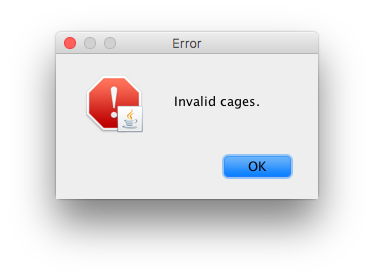
\includegraphics[scale=0.5]{Gambar/ImplementasiPengujian/InvalidCages.png}
\caption[Pesan error "\textit{Invalid cages}"]{Pesan error "\textit{Invalid cages}"}
\label{fig:invalidcages}
\end{figure}

Jika salah satu dari kedua error tersebut terjadi, maka akan keluar pesan error "\textit{Error in loading puzzle file}", seperti dapat dilihat pada Gambar~\ref{fig:errorinloadingpuzzlefile}.

\begin{figure}
\centering
\captionsetup{justification=centering}
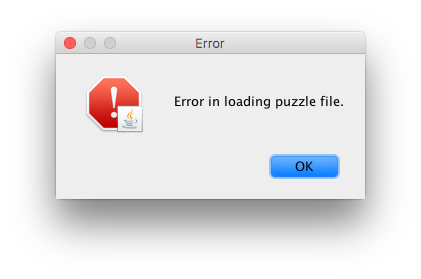
\includegraphics[scale=0.5]{Gambar/ImplementasiPengujian/Error.png}
\caption[Pesan error "\textit{Error in loading puzzle file}"]{Pesan error "\textit{Error in loading puzzle file}"}
\label{fig:errorinloadingpuzzlefile}
\end{figure}

\clearpage

\item Menyelesaikan permainan dengan usahanya sendiri

Jika pemain berhasil menyelesaikan permainan dengan usahanya sendiri, maka kotak informasi "\textit{Congratulations, you have successfully solved the puzzle}" akan muncul, seperti dapat dilihat pada Gambar~\ref{fig:congratulations}.

\begin{figure}
\centering
\captionsetup{justification=centering}
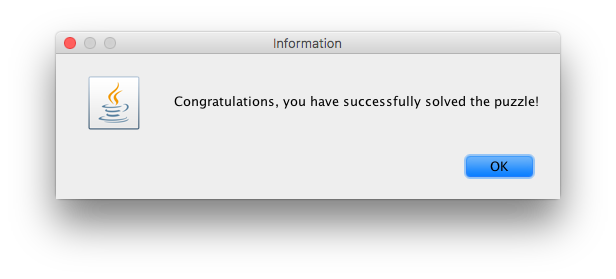
\includegraphics[scale=0.5]{Gambar/ImplementasiPengujian/Congratulations.png}
\caption[Pesan informasi "\textit{Congratulations, you have succesfully solved the puzzle}"]{Pesan informasi "\textit{Congratulations, you have succesfully solved the puzzle}"}
\label{fig:congratulations}
\end{figure}

\item Me-\textit{reset} permainan

Pemain dapat me-\textit{reset} permainan dengan memilih menu \textit{item} "\textit{Reset Puzzle}" dalam menu "\textit{File}". Jika menu \textit{item} ini dipilih, maka akan keluar kotak dialog "\textit{Are you sure you want to reset this puzzle?}, seperti dapat dilihat pada Gambar~\ref{fig:resetpuzzle}. Tekan tombol "\textit{Yes}" untuk me-\textit{reset} permainan, atau tekan tombol "\textit{No}" untuk membatalkan proses \textit{reset} permainan.

\begin{figure}
\centering
\captionsetup{justification=centering}
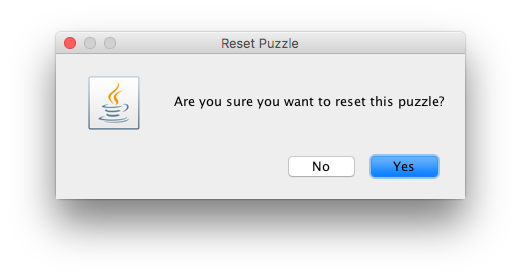
\includegraphics[scale=0.5]{Gambar/ImplementasiPengujian/ResetPuzzle.png}
\caption[Kotak dialog "\textit{Are you sure you want to reset this puzzle?}"]{Kotak dialog "\textit{Are you sure you want to reset this puzzle?}"}
\label{fig:resetpuzzle}
\end{figure}

\item Memeriksa permainan jika ada nilai yang salah di dalam \textit{grid}.

Perangkat lunak ini dapat memeriksa jika ada nilai yang salah di dalam \textit{grid} secara otomatis.

Jika ada nilai yang berulang dalam sebuah baris, maka akan keluar kotak informasi "\textit{Row} (nomor baris) \textit{has duplicate numbers}", seperti dapat dilihat pada Gambar~\ref{fig:rowduplicate}.

\begin{figure}
\centering
\captionsetup{justification=centering}
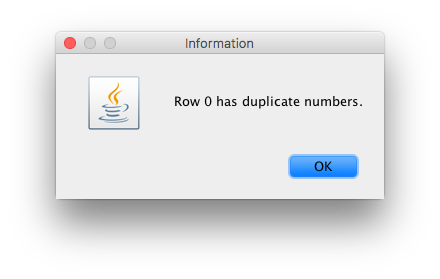
\includegraphics[scale=0.5]{Gambar/ImplementasiPengujian/RowDuplicate.png}
\caption[Pesan informasi "\textit{Row} (nomor baris) {has duplicate numbers}"]{Pesan informasi "\textit{Row} (nomor baris) \textit{has duplicate numbers}"}
\label{fig:rowduplicate}
\end{figure}

Jika ada nilai yang berulang dalam sebuah kolom, maka akan keluar kotak informasi "\textit{Column} (nomor kolom) \textit{has duplicate numbers}", seperti dapat dilihat pada Gambar~\ref{fig:columnduplicate}.

\begin{figure}
\centering
\captionsetup{justification=centering}
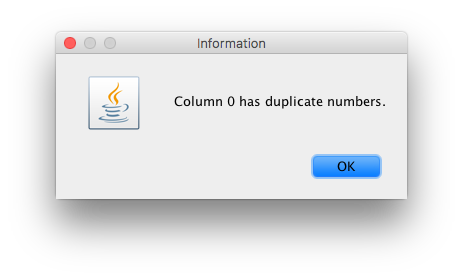
\includegraphics[scale=0.5]{Gambar/ImplementasiPengujian/ColumnDuplicate.png}
\caption[Pesan informasi "\textit{Column} (nomor kolom) {has duplicate numbers}"]{Pesan informasi "\textit{Column} (nomor kolom) \textit{has duplicate numbers}"}
\label{fig:columnduplicate}
\end{figure}

Jika nilai-nilai dalam sebuah \textit{cage} tidak mencapai nilai tujuan yang telah ditentukan jika dihitung dengan operasi matematika yang telah ditentukan, maka akan keluar kotak informasi "\textit{Values of cells in the cage do not reach the target number}", seperti dapat dilihat pada Gambar~\ref{fig:cagedonotreachtargetnumber}.

\begin{figure}
\centering
\captionsetup{justification=centering}
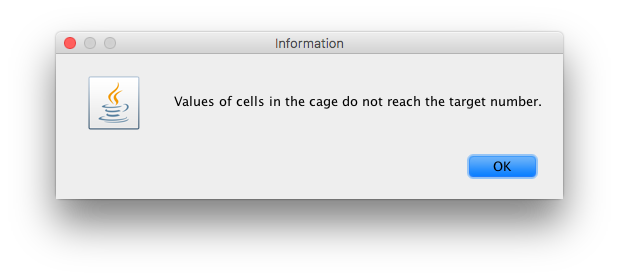
\includegraphics[scale=0.5]{Gambar/ImplementasiPengujian/CageDoNotReachTargetNumber.png}
\caption[Pesan informasi "\textit{Values of cells in the cage do not reach the target number}"]{Pesan informasi "\textit{Values of cells in the cage do not reach the target number}"}
\label{fig:cagedonotreachtargetnumber}
\end{figure}

Pemain juga dapat meminta perangkat lunak untuk memeriksa permainan jika ada nilai yang salah di dalam \textit{grid} secara manual, dengan memilih menu \textit{item} "\textit{Check Puzzle}" dalam menu "\textit{File}".

Jika menu \textit{item} ini dijalankan, dan ternyata ada nilai yang salah di dalam \textit{grid}, maka akan muncul kotak informasi "\textit{There are cells with incorrect values in the grid}", seperti dapat dilihat pada Gambar~\ref{fig:incorrectvalues}.

\begin{figure}
\centering
\captionsetup{justification=centering}
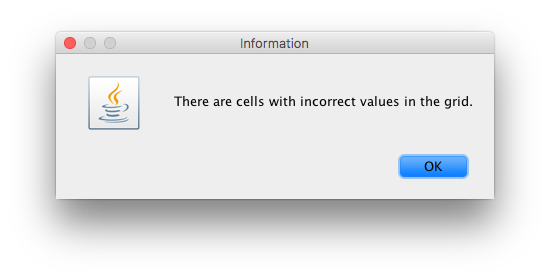
\includegraphics[scale=0.5]{Gambar/ImplementasiPengujian/IncorrectValues.png}
\caption[Pesan informasi "\textit{There are cells with incorrect values in the grid}"]{Pesan informasi "\textit{There are cells with incorrect values in the grid}"}
\label{fig:incorrectvalues}
\end{figure}

Jika menu \textit{item} ini dijalankan dan ternyata ada sel yang masih kosong, maka akan muncul kotak informasi "\textit{There are empty cells in the grid}", seperti dapat dilihat pada Gambar~\ref{fig:emptycells}.

\begin{figure}
\centering
\captionsetup{justification=centering}
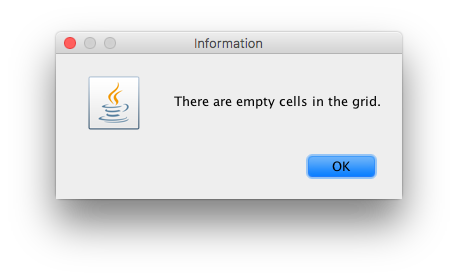
\includegraphics[scale=0.5]{Gambar/ImplementasiPengujian/EmptyCells.png}
\caption[Pesan informasi "\textit{There are empty cells in the grid}"]{Pesan informasi "\textit{There are empty cells in the grid}"}
\label{fig:emptycells}
\end{figure}

\item Menyelesaikan permainan dengan menggunakan algoritma \textit{backtracking}

Pemain dapat meminta perangkat lunak untuk menyelesaikan permainan dengan salah satu dari dua \textit{solver} yang disediakan. Salah satu dari kedua \textit{solver} tersebut adalah \textit{solver} dengan algoritma \textit{backtracking}. Untuk menggunakan \textit{solver} ini, pemain memilih menu \textit{item} "\textit{Backtracking}" dalam menu "\textit{Solve}".

Jika \textit{solver} ini berhasil dalam menyelesaikan permainan, maka akan muncul kotak informasi "\textit{The backtracking algorithm has successfully solved the puzzle}", dan waktu yang dibutuhkan oleh \textit{solver} untuk menyelesaikan permainan tersebut, seperti dapat dilihat pada Gambar~\ref{fig:backtrackingsuccess}.

\begin{figure}
\centering
\captionsetup{justification=centering}
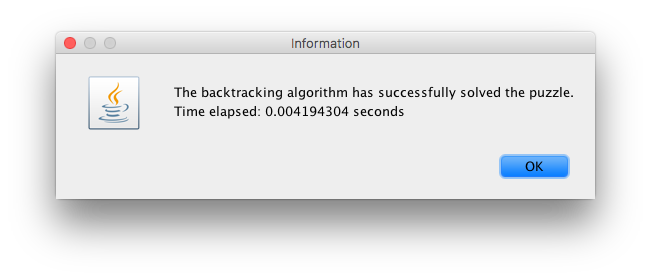
\includegraphics[scale=0.5]{Gambar/ImplementasiPengujian/BacktrackingSuccess.png}
\caption[Pesan informasi "\textit{The backtracking algorithm has successfully solved the puzzle}"]{Pesan informasi "\textit{The backtracking algorithm has successfully solved the puzzle}"}
\label{fig:backtrackingsuccess}
\end{figure}

Jika gagal, maka akan muncul kotak informasi "\textit{The backtracking algorithm has failed to solve the puzzle}", dan waktu yang dibutuhkan oleh \textit{solver} untuk menemukan bahwa tidak ada solusi untuk permainan tersebut, seperti dapat dilihat pada Gambar~\ref{fig:backtrackingfail}

\begin{figure}
\centering
\captionsetup{justification=centering}
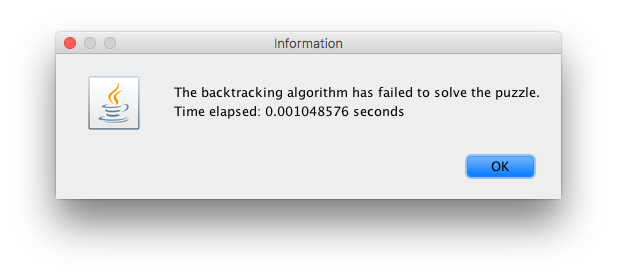
\includegraphics[scale=0.5]{Gambar/ImplementasiPengujian/BacktrackingFail.png}
\caption[Pesan informasi "\textit{The backtracking algorithm has failed to solve the puzzle}"]{Pesan informasi "\textit{The backtracking algorithm has failed to solve the puzzle}"}
\label{fig:backtrackingfail}
\end{figure}

\clearpage

\item Menyelesaikan permainan dengan menggunakan algoritma \textit{hybrid genetic}

Pemain dapat meminta perangkat lunak untuk menyelesaikan permainan dengan salah satu dari dua \textit{solver} yang disediakan. Salah satu dari kedua \textit{solver} tersebut adalah \textit{solver} dengan algoritma \textit{hybrid genetic}. Untuk menggunakan \textit{solver} ini, pemain memilih menu \textit{item} "\textit{Hybrid Genetic}" dalam menu "\textit{Solve}". Jika nilai untuk parameter-parameter algoritma genetik belum ditentukan, maka akan keluar pesan error "\textit{Genetic algorithm parameters have not been set}", seperti dapat dilihat pada Gambar~\ref{fig:gaparametershavenotbeenset}.

\begin{figure}
\centering
\captionsetup{justification=centering}
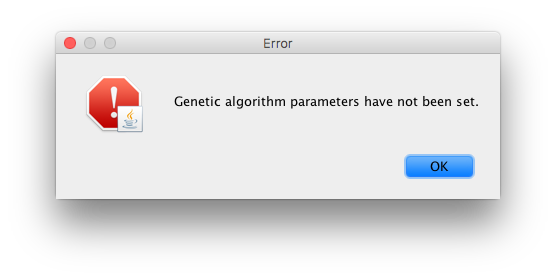
\includegraphics[scale=0.5]{Gambar/ImplementasiPengujian/GAParametersHaveNotBeenSet.png}
\caption[Pesan informasi "\textit{Genetic algorithm parameters have not been set}"]{Pesan informasi "\textit{Genetic algorithm parameters have not been set}"}
\label{fig:gaparametershavenotbeenset}
\end{figure}

Jika \textit{solver} ini berhasil dalam menyelesaikan permainan, maka akan muncul kotak informasi "\textit{The hybrid genetic algorithm has successfully solved the puzzle}", dan waktu yang dibutuhkan oleh \textit{solver} untuk menyelesaikan permainan tersebut, seperti dapat dilihat pada Gambar~\ref{fig:hybridgeneticsuccess}.

\begin{figure}
\centering
\captionsetup{justification=centering}
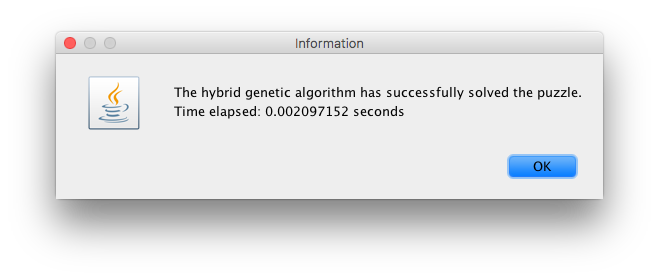
\includegraphics[scale=0.5]{Gambar/ImplementasiPengujian/HybridGeneticSuccess.png}
\caption[Pesan informasi "\textit{The hybrid genetic algorithm has successfully solved the puzzle}"]{Pesan informasi "\textit{The hybrid genetic algorithm has successfully solved the puzzle}"}
\label{fig:hybridgeneticsuccess}
\end{figure}

Jika gagal, maka akan muncul kotak informasi "\textit{The hybrid genetic algorithm has failed to solve the puzzle}", dan waktu yang dibutuhkan oleh \textit{solver} untuk menemukan bahwa tidak ada solusi untuk permainan tersebut, seperti dapat dilihat pada Gambar~\ref{fig:hybridgeneticfail}

\begin{figure}
\centering
\captionsetup{justification=centering}
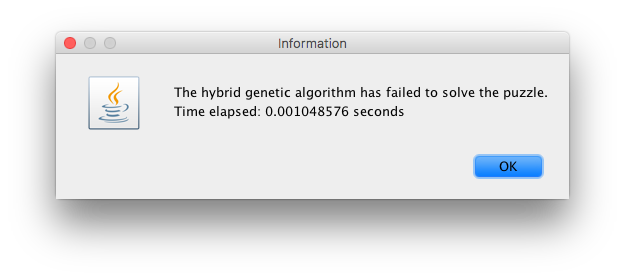
\includegraphics[scale=0.5]{Gambar/ImplementasiPengujian/HybridGeneticFail.png}
\caption[Pesan informasi "\textit{The hybrid genetic algorithm has failed to solve the puzzle}"]{Pesan informasi "\textit{The hybrid genetic algorithm has failed to solve the puzzle}"}
\label{fig:hybridgeneticfail}
\end{figure}

\item Mengatur nilai untuk parameter-parameter algoritma genetik

Pemain dapat mengatur sendiri nilai untuk parameter-parameter algoritma genetik dengan memilih menu \textit{item} "\textit{Set Genetic Algorithm Parameters}" dalam menu "\textit{Solve}". Akan muncul sebuah \textit{form} seperti dapat dilihat pada Gambar~\ref{fig:setgaparameters}.

\begin{figure}
\centering
\captionsetup{justification=centering}
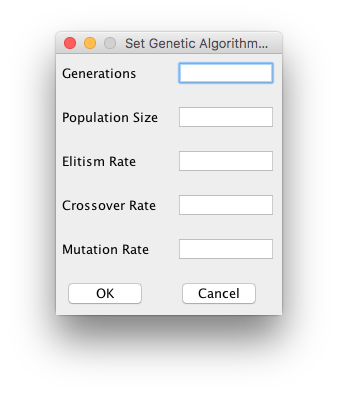
\includegraphics[scale=0.5]{Gambar/ImplementasiPengujian/SetGAParameters.png}
\caption[\textit{Form} untuk mengatur nilai untuk parameter-parameter algoritma genetik]{\textit{Form} untuk mengatur nilai untuk parameter-parameter algoritma genetik}
\label{fig:setgaparameters}
\end{figure}

Isilah \textit{form} tersebut dengan nilai yang diinginkan untuk setiap parameter algoritma genetik. Tekan tombol "\textit{OK}" untuk menyimpan nilai-nilai telah diisikan ke dalam \textit{form}, atau tekan tombol "\textit{Cancel}" untuk membatalkan proses mengatur nilai untuk parameter-parameter genetik. Jika angka yang dimasukkan ke dalam \textit{form} tidak \textit{valid}, maka akan muncul pesan error "\textit{Invalid number format}", seperti dapat dilihat pada Gambar~\ref{fig:invalidnumberformat}.

\begin{figure}
\centering
\captionsetup{justification=centering}
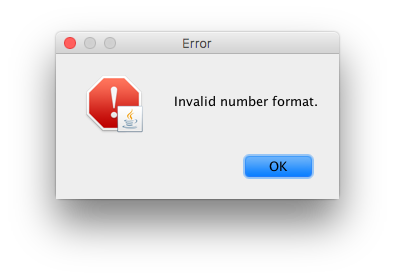
\includegraphics[scale=0.5]{Gambar/ImplementasiPengujian/InvalidNumberFormat.png}
\caption[Pesan error "\textit{Invalid number format}"]{Pesan error "\textit{Invalid number format}"}
\label{fig:invalidnumberformat}
\end{figure}

Jika jumlah dari tingkat \textit{elitism}, tingkat mutasi, dan tingkat kawin silang kurang dari 100\%, maka beberapa kromosom dari generasi sebelumnya akan diambil secara acak dan dimasukkan ke dalam generasi berikutnya sehingga jumlah kromosom dalam generasi berikutnya tetap sama. Jika jumlah dari tingkat \textit{elitism}, tingkat mutasi, dan tingkat kawin silang lebih dari 100\%, maka beberapa kromosom dari generasi berikutnya akan dibuang secara acak sehingga jumlah kromosom dalam generasi berikutnya tetap sama. 

\item Menutup \textit{file} permainan

Pemain dapat menutup \textit{file} permainan dengan memilih menu \textit{item} "\textit{Close Puzzle File}" dalam menu "\textit{File}". Jika menu \textit{item} ini dipilih, maka akan keluar kotak dialog "\textit{Are you sure you want to close this puzzle file?}, seperti dapat dilihat pada Gambar~\ref{fig:closepuzzlefile}. Tekan tombol "\textit{Yes}" untuk menutup \textit{file} permainan, atau tekan tombol "\textit{No}" untuk membatalkan proses menutup \textit{file} permainan.

\begin{figure}
\centering
\captionsetup{justification=centering}
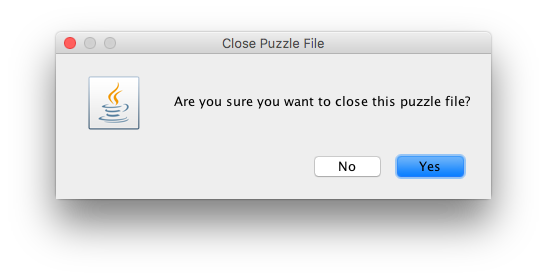
\includegraphics[scale=0.5]{Gambar/ImplementasiPengujian/ClosePuzzleFile.png}
\caption[Kotak dialog "\textit{Are you sure you want to close this puzzle file?}"]{Kotak dialog "\textit{Are you sure you want to close this puzzle file?}"}
\label{fig:closepuzzlefile}
\end{figure}

\item Menutup perangkat lunak

Pemain dapat menutup perangkat lunak dengan memilih menu \textit{item} "\textit{Exit}" dalam menu "\textit{File}". Jika menu \textit{item} ini dipilih, maka akan keluar kotak dialog "\textit{Are you sure you want to exit the application?}, seperti dapat dilihat pada Gambar~\ref{fig:exitapplication}. Tekan tombol "\textit{Yes}" untuk menutup perangkat lunak, atau tekan tombol "\textit{No}" untuk membatalkan proses menutup perangkat lunak.

\begin{figure}
\centering
\captionsetup{justification=centering}
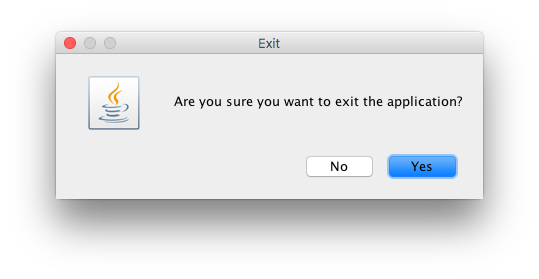
\includegraphics[scale=0.5]{Gambar/ImplementasiPengujian/Exit.png}
\caption[Kotak dialog "\textit{Are you sure you want to exit the application?}"]{Kotak dialog "\textit{Are you sure you want to exit the application?}"}
\label{fig:exitapplication}
\end{figure}

\end{enumerate}

\section{Pengujian Keakuratan}
\label{sec:pengujiankeakuratan}

Pengujian keakuratan dilakukan untuk memastikan bahwa permainan yang ditampilkan oleh perangkat lunak sesuai dengan \textit{file} permainan yang dibuka. Skenario-skenario yang akan dilakukan dalam pengujian keakuratan untuk perangkat lunak ini adalah:

\begin{enumerate}

\item Keakuratan dalam menerjemahkan isi \textit{file} masukan menjadi keluaran berupa GUI

Untuk menguji keakuratan perangkat lunak dalam menerjemahkan isi \textit{file} masukan menjadi keluaran berupa GUI, maka perangkat lunak akan diuji dengan membuka sebuah \textit{file} masukan, dan melihat apakah keluarannya, yaitu GUI-nya sesuai dengan \textit{file} masukan yang dibuka. 

Dalam kasus ini, perangkat lunak akan membuka \textit{file} masukan yang isinya dapat dilihat pada Gambar~\ref{fig:keakurataninput}.

\begin{figure}
\centering
\captionsetup{justification=centering}
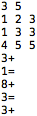
\includegraphics[scale=1]{Gambar/ImplementasiPengujian/Input.png}
\caption[\textit{File} masukan untuk pengujian keakuratan]{\textit{File} masukan untuk pengujian keakuratan}
\label{fig:keakurataninput}
\end{figure}

Perangkat lunak ini lalu menerjemahkan isi \textit{file} masukan menjadi keluaran berupa GUI yang dapat dilihat pada Gambar~\ref{fig:keakuratanoutput}.

\begin{figure}
\centering
\captionsetup{justification=centering}
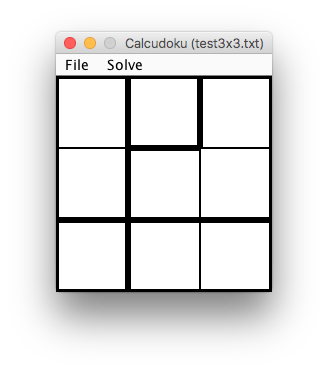
\includegraphics[scale=0.5]{Gambar/ImplementasiPengujian/Output1.png}
\caption[GUI permainan berdasarkan \textit{file} masukan yang dapat dilihat pada Gambar~\ref{fig:keakurataninput}]{GUI permainan berdasarkan \textit{file} masukan yang dapat dilihat pada Gambar~\ref{fig:keakurataninput}}
\label{fig:keakuratanoutput}
\end{figure}

Pada GUI ini, petunjuk, yaitu angka tujuan dan operasi matematika yang ditentukan untuk sebuah \textit{cage}, ditampilkan sebagai \textit{tooltip} yang akan muncul saat sel-sel yang berada di dalam sebuah \textit{cage} di-\textit{hover}. Setiap sel memilki \textit{tooltip} yang berisi petunjuk sesuai dengan \textit{cage} tempat sel tersebut berada. 

Dalam perangkat lunak ini, setiap sel sudah memiliki \textit{tooltip} sesuai dengan \textit{cage} tempat sel tersebut berada. 

Sel-sel dalam \textit{cage} 1, yaitu sel pada baris ke-1 dan kolom ke-1, dan sel pada baris ke-2 dan kolom ke-1, memiliki \textit{tooltip} "3+". Sel dalam \textit{cage} 2, yaitu sel pada baris ke-1 dan kolom ke-2, memiliki \textit{tooltip} "1=". Sel-sel dalam \textit{cage} 3, yaitu sel pada baris ke-1 dan kolom ke-3, sel pada baris ke-2 dan kolom ke-2, dan sel pada baris ke-2 dan kolom ke-3, memiliki \textit{tooltip} "8+". Sel dalam \textit{cage} 4, yaitu sel pada baris ke-3 dan kolom ke-1, memiliki \textit{tooltip} "3=". Sel-sel dalam \textit{cage} 5, yaitu sel pada baris ke-3 dan kolom ke-2, dan sel pada baris ke-3 dan kolom ke-3, memiliki \textit{tooltip} "3+".

\textit{Grid} dibatasi oleh garis tebal, setiap \textit{cage} dibatasi oleh garis tebal, dua sel yang berada di dalam dua \textit{cage} yang berbeda dibatasi oleh garis tebal, dan dua sel yang berada di dalam \textit{cage} yang sama dibatasi oleh garis tipis. 

Dalam perangkat lunak ini, \textit{grid} dan setiap sel sudah memiliki garis pembatas yang tepat. \textit{Grid} dibatasi oleh garis tebal.

Pada baris ke-1, sel pada kolom ke-1 dan kolom ke-2 dibatasi oleh garis tebal karena kedua sel tersebut berada dalam dua \textit{cage} yang berbeda, sel pada kolom ke-2 dan kolom ke-3 dibatasi oleh garis tebal karena kedua sel tersebut berada dalam dua \textit{cage} yang berbeda. Pada baris ke-2, sel pada kolom ke-1 dan kolom ke-2 dibatasi oleh garis tebal karena kedua sel tersebut berada dalam dua \textit{cage} yang berbeda, sel pada kolom ke-2 dan kolom ke-3 dibatasi oleh garis tipis karena kedua sel tersebut berada dalam dua \textit{cage} yang sama. Pada baris ke-3, sel pada kolom ke-1 dan kolom ke-2 dibatasi oleh garis tebal karena kedua sel tersebut berada dalam dua \textit{cage} yang berbeda, sel pada kolom ke-2 dan kolom ke-3 dibatasi oleh garis tipis karena kedua sel tersebut berada dalam dua \textit{cage} yang sama.

Pada kolom ke-1, sel pada baris ke-1 dan baris ke-2 dibatasi oleh garis tips karena kedua sel tersebut berada dalam dua \textit{cage} yang sama, sel pada baris ke-2 dan baris ke-3 dibatasi oleh garis tebal karena kedua sel tersebut berada dalam dua \textit{cage} yang berbeda.Pada kolom ke-2, sel pada baris ke-1 dan baris ke-2 dibatasi oleh garis tebal karena kedua sel tersebut berada dalam dua \textit{cage} yang berbeda, sel pada baris ke-2 dan baris ke-3 dibatasi oleh garis tebal karena kedua sel tersebut berada dalam dua \textit{cage} yang berbeda. Pada kolom ke-3, sel pada baris ke-1 dan baris ke-2 dibatasi oleh garis tipis karena kedua sel tersebut berada dalam dua \textit{cage} yang sama, sel pada baris ke-2 dan baris ke-3 dibatasi oleh garis tebal karena kedua sel tersebut berada dalam dua \textit{cage} yang berbeda.

\item Keakuratan dalam menampilkan pesan informasi pada waktunya.

Untuk menguji keakuratan perangkat lunak dalam menampilkan pesan informasi pada waktunya, maka perangkat lunak harus diuji dengan menyelesaikan sebuah permainan, dan melihat apa kotak informasi ditampilkan pada waktunya atau tidak.

Dalam kasus ini, permainan berdasarkan \textit{file} yang isinya ditampilkan pada Gambar~\ref{fig:keakurataninput} akan diselesaikan.

\textit{Cage} 2, yang hanya berukuran satu sel yang terletak pada baris ke-1 dan kolom ke-2, dan memiliki petunjuk "1\begin{math}=\end{math}". Isilah sel tersebut dengan angka 2. Karena 2 bukan angka tujuan dari \textit{cage} tersebut, maka pesan informasi "\textit{Values of cells in the cage do not reach the target number}" seperti yang dapat dilihat pada Gambar~\ref{fig:cagedonotreachtargetnumber} akan muncul. Hapuslah angka 2 dari sel tersebut, dan isilah dengan angka 1, yang merupakan angka tujuan dari \textit{cage} tersebut. 

Isilah sel pada baris ke-1 dan kolom ke-1 dengan angka 1. Karena ada angka yang berulang dalam satu baris, maka pesan informasi "\textit{Row has duplicate numbers}" seperti yang dapat dilihat pada Gambar~\ref{fig:rowduplicate} akan muncul. Hapuslah angka 1 dari sel tersebut. Sekarang isilah sel pada baris ke-1 dan kolom ke-1 dengan angka 1. Karena ada angka yang berulang dalam satu baris, maka pesan informasi "\textit{Row has duplicate numbers}" seperti yang dapat dilihat pada Gambar~\ref{fig:rowduplicate} akan muncul. Hapuslah angka 1 dari sel tersebut.

Isilah sel pada baris ke-2 dan kolom ke-2 dengan angka 1. Karena ada angka yang berulang dalam satu kolom, maka pesan informasi "\textit{Column has duplicate numbers}" seperti yang dapat dilihat pada Gambar~\ref{fig:columnduplicate} akan muncul. Hapuslah angka 1 dari sel tersebut.

Selesaikan permainan ini dengan mengisi sel-sel lainnya dengan angka yang benar. Solusi dari permainan ini dapat dilihat pada Gambar~\ref{fig:keakuratansolusi}.

\begin{figure}
\centering
\captionsetup{justification=centering}
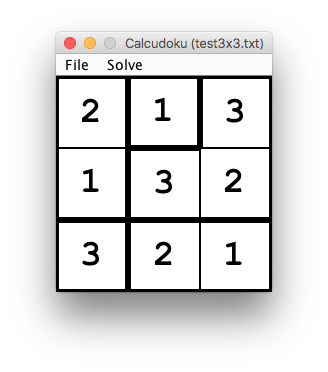
\includegraphics[scale=0.5]{Gambar/ImplementasiPengujian/Output2.png}
\caption[Solusi untuk permainan berdasarkan \textit{file} masukan yang dapat dilihat pada Gambar~\ref{fig:keakurataninput}]{Solusi untuk permainan berdasarkan \textit{file} masukan yang dapat dilihat pada Gambar~\ref{fig:keakurataninput}}
\label{fig:keakuratansolusi}
\end{figure}

Setelah mengisi seluruh sel di dalam \textit{grid} sesuai dengan solusi tersebut, maka pesan informasi "\textit{Congratulations, you have successfully solved the puzzle}" seperti yang dapat dilihat pada Gambar~\ref{fig:congratulations} akan muncul.

Perangkat lunak ini telah berhasil memunculkan pesan informasi pada waktunya.

\end{enumerate}

\section{Pengujian Algoritma \textit{Backtracking}}
\label{sec:pengujianbacktracking}

Pengujian algoritma \textit{backtracking} untuk Calcudoku dilakukan untuk mengetahui keberhasilan dan kecepatan algoritma \textit{backtracking} dalam menyelesaikan permainan Calcudoku.

\begin{table}
\centering
\captionsetup{justification=centering}
\caption[Hasil pengujian algoritma \textit{backtracking} untuk Calcudoku]{Hasil pengujian algoritma \textit{backtracking} untuk Calcudoku}
\begin{tabular}{| l | l | l |}
\hline
Ukuran \textit{Grid} & Tingkat Keberhasilan & Kecepatan \\
\hline \hline
\begin{math}4 \times 4\end{math} & 100\% & 0.067 detik \\
\hline
\begin{math}5 \times 5\end{math} & 100\% & 0.701 detik \\
\hline
\begin{math}6 \times 6\end{math} & 100\% & 13.84 detik \\
\hline
\begin{math}7 \times 7\end{math} & 100\% & 482.653 detik \\
\hline
\begin{math}8 \times 8\end{math} & 100\% & 2134.655 detik \\
\hline
\end{tabular}
\label{tab:pengujianbt}
\end{table}

Berdasarkan hasil pengujian yang dapat dilihat pada Tabel~\ref{tab:pengujianbt}, algoritma \textit{backtracking} dapat menyelesaikan semua permainan yang diujikan. Semakin besar ukuran \textit{grid}, maka waktu yang dibutuhkan oleh algoritma \textit{backtracking} untuk menyelesaikan permainan semakin lama. Pada ukuran \textit{grid} yang besar, algoritma \textit{backtracking} sangat lambat dalam menyelesaikan permainan.

Hasil pengujian selengkapnya dapat dilihat pada Lampiran~\ref{chap:hasilpengujian}.

\section{Pengujian dan Eksperimen Algoritma \textit{Hybrid Genetic}}
\label{sec:pengujianhybridgenetic}

Pengujian algoritma \textit{hybrid genetic} untuk Calcudoku dilakukan untuk mengetahui keberhasilan dan kecepatan algoritma \textit{hybrid genetic} dalam menyelesaikan permainan Calcudoku.

Pada algoritma \textit{backtracking} tidak ada parameter yang nilainya dapat diubah, sedangkan pada algoritma \textit{hybrid genetic}, nilai dari parameter-parameter untuk algoritma genetik dapat diubah. Tidak ada nilai \textit{default} untuk parameter-parameter dari algoritma genetik ini. Nilai dari parameter-parameter tersebut harus diisi sendiri oleh pemain.

Dalam kasus ini, pengujian eksperimental dilakukan dengan melakukan pengujian keberhasilan dan kecepatan dari \textit{solver} dengan algoritma \textit{hybrid genetic} dengan mengatur nilai dari parameter-parameter dari algoritma genetik dengan nilai yang berbeda-beda untuk setiap percobaan.

Terdapat 16 skenario yang dilakukan untuk percobaan ini. Nilai untuk parameter-parameter untuk algoritma genetik untuk setiap percobaan yang dilakukan dapat dilihat pada Tabel~\ref{tab:nilaiparameterhg}.

\begin{table}
\centering
\captionsetup{justification=centering}
\caption[Nilai untuk parameter-parameter algoritma genetik untuk setiap percobaan yang dilakukan]{Nilai untuk parameter-parameter algoritma genetik untuk setiap percobaan yang dilakukan}
\begin{tabular}{| l | l | l | l | l | l |}
\hline
Skenario & Populasi & Generasi & \textit{Elitism} & Mutasi & Kawin Silang  \\
\hline \hline
1 & 1000 & 100 & 10\% & 10\% & 80\% \\
\hline
2 & 1000 & 100 & 5\% & 10\% & 85\% \\
\hline
3 & 1000 & 100 & 10\% & 5\% & 85\% \\
\hline
4 & 1000 & 100  & 5\% & 5\% & 90\% \\
\hline
5 & 100 & 100 & 10\% & 10\% & 80\% \\
\hline
6 & 100 & 100 & 5\% & 10\% & 85\% \\
\hline
7 & 100 & 100 & 10\% & 5\% & 85\% \\
\hline
8 & 100 & 100 & 5\% & 5\% & 90\% \\
\hline
9 & 1000 & 10 & 10\% & 10\% & 80\% \\
\hline
10 & 1000 & 10 & 5\% & 10\% & 85\% \\
\hline
11 & 1000 & 10 & 10\% & 5\% & 85\% \\
\hline
12 & 1000 & 10  & 5\% & 5\% & 90\% \\
\hline
13 & 100 & 10 & 10\% & 10\% & 80\% \\
\hline
14 & 100 & 10 & 5\% & 10\% & 85\% \\
\hline
15 & 100 & 10 & 10\% & 5\% & 85\% \\
\hline
16 & 100 & 10 & 5\% & 5\% & 90\% \\
\hline
\end{tabular}
\label{tab:nilaiparameterhg}
\end{table}

\subsection{Skenario 1}
\label{sec:skenario1}

Hasil pengujian Skenario 1 dapat dilihat pada Tabel~\ref{tab:pengujianhg1}.

\begin{table}
\centering
\captionsetup{justification=centering}
\caption[Hasil pengujian algoritma \textit{hybrid genetic} untuk Calcudoku (Skenario 1)]{Hasil pengujian algoritma \textit{hybrid genetic} untuk Calcudoku (Skenario 1)}
\begin{tabular}{| l | l | l | l |}
\hline
Ukuran \textit{Grid} & \makecell[l]{Rata-Rata \\ Tingkat Keberhasilan} & \makecell[l]{Rata-Rata \\ Kecepatan} & \makecell[l]{Rata-Rata \\ Jumlah Sel Diisi Algoritma \textit{Rule Based}} \\
\hline \hline
\begin{math}4 \times 4\end{math} & 100\% & 3.579 detik & 3 \\
\hline
\begin{math}5 \times 5\end{math} & 42.308\% & 8.389 detik & 9 \\
\hline
\begin{math}6 \times 6\end{math} & 0\% & - & - \\
\hline
\begin{math}7 \times 7\end{math} & 0\% & - & - \\
\hline
\begin{math}8 \times 8\end{math} & 0\% & - & - \\
\hline
\end{tabular}
\label{tab:pengujianhg1}
\end{table}

\clearpage

\subsection{Skenario 2}
\label{sec:skenario2}

Hasil pengujian Skenario 2 dapat dilihat pada Tabel~\ref{tab:pengujianhg2}.

\begin{table}
\centering
\captionsetup{justification=centering}
\caption[Hasil pengujian algoritma \textit{hybrid genetic} untuk Calcudoku (Skenario 2)]{Hasil pengujian algoritma \textit{hybrid genetic} untuk Calcudoku (Skenario 2)}
\begin{tabular}{| l | l | l | l |}
\hline
Ukuran \textit{Grid} & \makecell[l]{Rata-Rata \\ Tingkat Keberhasilan} & \makecell[l]{Rata-Rata \\ Kecepatan} & \makecell[l]{Rata-Rata \\ Jumlah Sel Diisi Algoritma \textit{Rule Based}} \\
\hline \hline
\begin{math}4 \times 4\end{math} & 100\% & 4.002 detik & 3 \\
\hline
\begin{math}5 \times 5\end{math} & 42.308\% & 9.258 detik & 9 \\
\hline
\begin{math}6 \times 6\end{math} & 0\% & - & - \\
\hline
\begin{math}7 \times 7\end{math} & 0\% & - & - \\
\hline
\begin{math}8 \times 8\end{math} & 0\% & - & - \\
\hline
\end{tabular}
\label{tab:pengujianhg2}
\end{table}

\subsection{Skenario 3}
\label{sec:skenario3}

Hasil pengujian Skenario 3 dapat dilihat pada Tabel~\ref{tab:pengujianhg3}.

\begin{table}
\centering
\captionsetup{justification=centering}
\caption[Hasil pengujian algoritma \textit{hybrid genetic} untuk Calcudoku (Skenario 3)]{Hasil pengujian algoritma \textit{hybrid genetic} untuk Calcudoku (Skenario 3)}
\begin{tabular}{| l | l | l | l |}
\hline
Ukuran \textit{Grid} & \makecell[l]{Rata-Rata \\ Tingkat Keberhasilan} & \makecell[l]{Rata-Rata \\ Kecepatan} & \makecell[l]{Rata-Rata \\ Jumlah Sel Diisi Algoritma \textit{Rule Based}} \\
\hline \hline
\begin{math}4 \times 4\end{math} & 100\% & 3.751 detik & 3 \\
\hline
\begin{math}5 \times 5\end{math} & 42.308\% & 8.806 detik & 9 \\
\hline
\begin{math}6 \times 6\end{math} & 0\% & - & - \\
\hline
\begin{math}7 \times 7\end{math} & 0\% & - & - \\
\hline
\begin{math}8 \times 8\end{math} & 0\% & - & - \\
\hline
\end{tabular}
\label{tab:pengujianhg3}
\end{table}

\subsection{Skenario 4}
\label{sec:skenario4}

Hasil pengujian Skenario 4 dapat dilihat pada Tabel~\ref{tab:pengujianhg4}.

\begin{table}
\centering
\captionsetup{justification=centering}
\caption[Hasil pengujian algoritma \textit{hybrid genetic} untuk Calcudoku (Skenario 4)]{Hasil pengujian algoritma \textit{hybrid genetic} untuk Calcudoku (Skenario 4)}
\begin{tabular}{| l | l | l | l |}
\hline
Ukuran \textit{Grid} & \makecell[l]{Rata-Rata \\ Tingkat Keberhasilan} & \makecell[l]{Rata-Rata \\ Kecepatan} & \makecell[l]{Rata-Rata \\ Jumlah Sel Diisi Algoritma \textit{Rule Based}} \\
\hline \hline
\begin{math}4 \times 4\end{math} & 100\% & 4.175 detik & 3 \\
\hline
\begin{math}5 \times 5\end{math} & 42.308\% & 9.676 detik & 9 \\
\hline
\begin{math}6 \times 6\end{math} & 0\% & - & - \\
\hline
\begin{math}7 \times 7\end{math} & 0\% & - & - \\
\hline
\begin{math}8 \times 8\end{math} & 0\% & - & - \\
\hline
\end{tabular}
\label{tab:pengujianhg4}
\end{table}

\clearpage

\subsection{Skenario 5}
\label{sec:skenario5}

Hasil pengujian Skenario 5 dapat dilihat pada Tabel~\ref{tab:pengujianhg5}.

\begin{table}
\centering
\captionsetup{justification=centering}
\caption[Hasil pengujian algoritma \textit{hybrid genetic} untuk Calcudoku (Skenario 5)]{Hasil pengujian algoritma \textit{hybrid genetic} untuk Calcudoku (Skenario 5)}
\begin{tabular}{| l | l | l | l |}
\hline
Ukuran \textit{Grid} & \makecell[l]{Rata-Rata \\ Tingkat Keberhasilan} & \makecell[l]{Rata-Rata \\ Kecepatan} & \makecell[l]{Rata-Rata \\ Jumlah Sel Diisi Algoritma \textit{Rule Based}} \\
\hline \hline
\begin{math}4 \times 4\end{math} & 61.538\% & 0.498 detik & 5 \\
\hline
\begin{math}5 \times 5\end{math} & 19.231\% & 0.311 detik & 14 \\
\hline
\begin{math}6 \times 6\end{math} & 0\% & - & - \\
\hline
\begin{math}7 \times 7\end{math} & 0\% & - & - \\
\hline
\begin{math}8 \times 8\end{math} & 0\% & - & - \\
\hline
\end{tabular}
\label{tab:pengujianhg5}
\end{table}

\subsection{Skenario 6}
\label{sec:skenario6}

Hasil pengujian Skenario 6 dapat dilihat pada Tabel~\ref{tab:pengujianhg5}.

\begin{table}
\centering
\captionsetup{justification=centering}
\caption[Hasil pengujian algoritma \textit{hybrid genetic} untuk Calcudoku (Skenario 6)]{Hasil pengujian algoritma \textit{hybrid genetic} untuk Calcudoku (Skenario 6)}
\begin{tabular}{| l | l | l | l |}
\hline
Ukuran \textit{Grid} & \makecell[l]{Rata-Rata \\ Tingkat Keberhasilan} & \makecell[l]{Rata-Rata \\ Kecepatan} & \makecell[l]{Rata-Rata \\ Jumlah Sel Diisi Algoritma \textit{Rule Based}} \\
\hline \hline
\begin{math}4 \times 4\end{math} & 61.538\% & 0.553 detik & 5 \\
\hline
\begin{math}5 \times 5\end{math} & 19.231\% & 0.339 detik & 14 \\
\hline
\begin{math}6 \times 6\end{math} & 0\% & - & - \\
\hline
\begin{math}7 \times 7\end{math} & 0\% & - & - \\
\hline
\begin{math}8 \times 8\end{math} & 0\% & - & - \\
\hline
\end{tabular}
\label{tab:pengujianhg6}
\end{table}

\subsection{Skenario 7}
\label{sec:skenario7}

Hasil pengujian Skenario 7 dapat dilihat pada Tabel~\ref{tab:pengujianhg7}.

\begin{table}
\centering
\captionsetup{justification=centering}
\caption[Hasil pengujian algoritma \textit{hybrid genetic} untuk Calcudoku (Skenario 7)]{Hasil pengujian algoritma \textit{hybrid genetic} untuk Calcudoku (Skenario 7)}
\begin{tabular}{| l | l | l | l |}
\hline
Ukuran \textit{Grid} & \makecell[l]{Rata-Rata \\ Tingkat Keberhasilan} & \makecell[l]{Rata-Rata \\ Kecepatan} & \makecell[l]{Rata-Rata \\ Jumlah Sel Diisi Algoritma \textit{Rule Based}} \\
\hline \hline
\begin{math}4 \times 4\end{math} & 61.538\% & 0.524 detik & 5 \\
\hline
\begin{math}5 \times 5\end{math} & 19.231\% & 0.325 detik & 14 \\
\hline
\begin{math}6 \times 6\end{math} & 0\% & - & - \\
\hline
\begin{math}7 \times 7\end{math} & 0\% & - & - \\
\hline
\begin{math}8 \times 8\end{math} & 0\% & - & - \\
\hline
\end{tabular}
\label{tab:pengujianhg7}
\end{table}

\clearpage

\subsection{Skenario 8}
\label{sec:skenario8}

Hasil pengujian Skenario 8 dapat dilihat pada Tabel~\ref{tab:pengujianhg8}.

\begin{table}
\centering
\captionsetup{justification=centering}
\caption[Hasil pengujian algoritma \textit{hybrid genetic} untuk Calcudoku (Skenario 8)]{Hasil pengujian algoritma \textit{hybrid genetic} untuk Calcudoku (Skenario 8)}
\begin{tabular}{| l | l | l | l |}
\hline
Ukuran \textit{Grid} & \makecell[l]{Rata-Rata \\ Tingkat Keberhasilan} & \makecell[l]{Rata-Rata \\ Kecepatan} & \makecell[l]{Rata-Rata \\ Jumlah Sel Diisi Algoritma \textit{Rule Based}} \\
\hline \hline
\begin{math}4 \times 4\end{math} & 61.538\% & 0.579 detik & 5 \\
\hline
\begin{math}5 \times 5\end{math} & 19.231\% & 0.352 detik & 14 \\
\hline
\begin{math}6 \times 6\end{math} & 0\% & - & - \\
\hline
\begin{math}7 \times 7\end{math} & 0\% & - & - \\
\hline
\begin{math}8 \times 8\end{math} & 0\% & - & - \\
\hline
\end{tabular}
\label{tab:pengujianhg8}
\end{table}

\subsection{Skenario 9}
\label{sec:skenario9}

Hasil pengujian Skenario 9 dapat dilihat pada Tabel~\ref{tab:pengujianhg9}.

\begin{table}
\centering
\captionsetup{justification=centering}
\caption[Hasil pengujian algoritma \textit{hybrid genetic} untuk Calcudoku (Skenario 9)]{Hasil pengujian algoritma \textit{hybrid genetic} untuk Calcudoku (Skenario 9)}
\begin{tabular}{| l | l | l | l |}
\hline
Ukuran \textit{Grid} & \makecell[l]{Rata-Rata \\ Tingkat Keberhasilan} & \makecell[l]{Rata-Rata \\ Kecepatan} & \makecell[l]{Rata-Rata \\ Jumlah Sel Diisi Algoritma \textit{Rule Based}} \\
\hline \hline
\begin{math}4 \times 4\end{math} & 35.897\% & 0.511 detik & 7 \\
\hline
\begin{math}5 \times 5\end{math} & 15.385\% & 0.487 detik & 15 \\
\hline
\begin{math}6 \times 6\end{math} & 0\% & - & - \\
\hline
\begin{math}7 \times 7\end{math} & 0\% & - & - \\
\hline
\begin{math}8 \times 8\end{math} & 0\% & - & - \\
\hline
\end{tabular}
\label{tab:pengujianhg9}
\end{table}

\subsection{Skenario 10}
\label{sec:skenario10}

Hasil pengujian Skenario 10 dapat dilihat pada Tabel~\ref{tab:pengujianhg10}.

\begin{table}
\centering
\captionsetup{justification=centering}
\caption[Hasil pengujian algoritma \textit{hybrid genetic} untuk Calcudoku (Skenario 10)]{Hasil pengujian algoritma \textit{hybrid genetic} untuk Calcudoku (Skenario 10)}
\begin{tabular}{| l | l | l | l |}
\hline
Ukuran \textit{Grid} & \makecell[l]{Rata-Rata \\ Tingkat Keberhasilan} & \makecell[l]{Rata-Rata \\ Kecepatan} & \makecell[l]{Rata-Rata \\ Jumlah Sel Diisi Algoritma \textit{Rule Based}} \\
\hline \hline
\begin{math}4 \times 4\end{math} & 35.897\% & 0.511 detik & 7 \\
\hline
\begin{math}5 \times 5\end{math} & 15.385\% & 0.487 detik & 15 \\
\hline
\begin{math}6 \times 6\end{math} & 0\% & - & - \\
\hline
\begin{math}7 \times 7\end{math} & 0\% & - & - \\
\hline
\begin{math}8 \times 8\end{math} & 0\% & - & - \\
\hline
\end{tabular}
\label{tab:pengujianhg10}
\end{table}

\clearpage

\subsection{Skenario 11}
\label{sec:skenario11}

Hasil pengujian Skenario 11 dapat dilihat pada Tabel~\ref{tab:pengujianhg11}.

\begin{table}
\centering
\captionsetup{justification=centering}
\caption[Hasil pengujian algoritma \textit{hybrid genetic} untuk Calcudoku (Skenario 11)]{Hasil pengujian algoritma \textit{hybrid genetic} untuk Calcudoku (Skenario 11)}
\begin{tabular}{| l | l | l | l |}
\hline
Ukuran \textit{Grid} & \makecell[l]{Rata-Rata \\ Tingkat Keberhasilan} & \makecell[l]{Rata-Rata \\ Kecepatan} & \makecell[l]{Rata-Rata \\ Jumlah Sel Diisi Algoritma \textit{Rule Based}} \\
\hline \hline
\begin{math}4 \times 4\end{math} & 35.897\% & 0.511 detik & 7 \\
\hline
\begin{math}5 \times 5\end{math} & 15.385\% & 0.487 detik & 15 \\
\hline
\begin{math}6 \times 6\end{math} & 0\% & - & - \\
\hline
\begin{math}7 \times 7\end{math} & 0\% & - & - \\
\hline
\begin{math}8 \times 8\end{math} & 0\% & - & - \\
\hline
\end{tabular}
\label{tab:pengujianhg11}
\end{table}

\subsection{Skenario 12}
\label{sec:skenario12}

Hasil pengujian Skenario 12 dapat dilihat pada Tabel~\ref{tab:pengujianhg12}.

\begin{table}
\centering
\captionsetup{justification=centering}
\caption[Hasil pengujian algoritma \textit{hybrid genetic} untuk Calcudoku (Skenario 12)]{Hasil pengujian algoritma \textit{hybrid genetic} untuk Calcudoku (Skenario 12)}
\begin{tabular}{| l | l | l | l |}
\hline
Ukuran \textit{Grid} & \makecell[l]{Rata-Rata \\ Tingkat Keberhasilan} & \makecell[l]{Rata-Rata \\ Kecepatan} & \makecell[l]{Rata-Rata \\ Jumlah Sel Diisi Algoritma \textit{Rule Based}} \\
\hline \hline
\begin{math}4 \times 4\end{math} & 35.897\% & 0.511 detik & 7 \\
\hline
\begin{math}5 \times 5\end{math} & 15.385\% & 0.487 detik & 15 \\
\hline
\begin{math}6 \times 6\end{math} & 0\% & - & - \\
\hline
\begin{math}7 \times 7\end{math} & 0\% & - & - \\
\hline
\begin{math}8 \times 8\end{math} & 0\% & - & - \\
\hline
\end{tabular}
\label{tab:pengujianhg12}
\end{table}

\subsection{Skenario 13}
\label{sec:skenario13}

Hasil pengujian Skenario 13 dapat dilihat pada Tabel~\ref{tab:pengujianhg13}.

\begin{table}
\centering
\captionsetup{justification=centering}
\caption[Hasil pengujian algoritma \textit{hybrid genetic} untuk Calcudoku (Skenario 13)]{Hasil pengujian algoritma \textit{hybrid genetic} untuk Calcudoku (Skenario 13)}
\begin{tabular}{| l | l | l | l |}
\hline
Ukuran \textit{Grid} & \makecell[l]{Rata-Rata \\ Tingkat Keberhasilan} & \makecell[l]{Rata-Rata \\ Kecepatan} & \makecell[l]{Rata-Rata \\ Jumlah Sel Diisi Algoritma \textit{Rule Based}} \\
\hline \hline
\begin{math}4 \times 4\end{math} & 23.077\% & 0.054 detik & 9 \\
\hline
\begin{math}5 \times 5\end{math} & 15.385\% & 0.077 detik & 15 \\
\hline
\begin{math}6 \times 6\end{math} & 0\% & - & - \\
\hline
\begin{math}7 \times 7\end{math} & 0\% & - & - \\
\hline
\begin{math}8 \times 8\end{math} & 0\% & - & - \\
\hline
\end{tabular}
\label{tab:pengujianhg13}
\end{table}

\clearpage

\subsection{Skenario 14}
\label{sec:skenario14}

Hasil pengujian Skenario 14 dapat dilihat pada Tabel~\ref{tab:pengujianhg14}.

\begin{table}
\centering
\captionsetup{justification=centering}
\caption[Hasil pengujian algoritma \textit{hybrid genetic} untuk Calcudoku (Skenario 14)]{Hasil pengujian algoritma \textit{hybrid genetic} untuk Calcudoku (Skenario 14)}
\begin{tabular}{| l | l | l | l |}
\hline
Ukuran \textit{Grid} & \makecell[l]{Rata-Rata \\ Tingkat Keberhasilan} & \makecell[l]{Rata-Rata \\ Kecepatan} & \makecell[l]{Rata-Rata \\ Jumlah Sel Diisi Algoritma \textit{Rule Based}} \\
\hline \hline
\begin{math}4 \times 4\end{math} & 23.077\% & 0.054 detik & 9 \\
\hline
\begin{math}5 \times 5\end{math} & 15.385\% & 0.077 detik & 15 \\
\hline
\begin{math}6 \times 6\end{math} & 0\% & - & - \\
\hline
\begin{math}7 \times 7\end{math} & 0\% & - & - \\
\hline
\begin{math}8 \times 8\end{math} & 0\% & - & - \\
\hline
\end{tabular}
\label{tab:pengujianhg14}
\end{table}

\subsection{Skenario 15}
\label{sec:skenario15}

Hasil pengujian Skenario 15 dapat dilihat pada Tabel~\ref{tab:pengujianhg15}.

\begin{table}
\centering
\captionsetup{justification=centering}
\caption[Hasil pengujian algoritma \textit{hybrid genetic} untuk Calcudoku (Skenario 15)]{Hasil pengujian algoritma \textit{hybrid genetic} untuk Calcudoku (Skenario 15)}
\begin{tabular}{| l | l | l | l |}
\hline
Ukuran \textit{Grid} & \makecell[l]{Rata-Rata \\ Tingkat Keberhasilan} & \makecell[l]{Rata-Rata \\ Kecepatan} & \makecell[l]{Rata-Rata \\ Jumlah Sel Diisi Algoritma \textit{Rule Based}} \\
\hline \hline
\begin{math}4 \times 4\end{math} & 23.077\% & 0.054 detik & 9 \\
\hline
\begin{math}5 \times 5\end{math} & 15.385\% & 0.077 detik & 15 \\
\hline
\begin{math}6 \times 6\end{math} & 0\% & - & - \\
\hline
\begin{math}7 \times 7\end{math} & 0\% & - & - \\
\hline
\begin{math}8 \times 8\end{math} & 0\% & - & - \\
\hline
\end{tabular}
\label{tab:pengujianhg15}
\end{table}

\subsection{Skenario 16}
\label{sec:skenario16}

Hasil pengujian Skenario 16 dapat dilihat pada Tabel~\ref{tab:pengujianhg16}.

\begin{table}
\centering
\captionsetup{justification=centering}
\caption[Hasil pengujian algoritma \textit{hybrid genetic} untuk Calcudoku (Skenario 16)]{Hasil pengujian algoritma \textit{hybrid genetic} untuk Calcudoku (Skenario 16)}
\begin{tabular}{| l | l | l | l |}
\hline
Ukuran \textit{Grid} & \makecell[l]{Rata-Rata \\ Tingkat Keberhasilan} & \makecell[l]{Rata-Rata \\ Kecepatan} & \makecell[l]{Rata-Rata \\ Jumlah Sel Diisi Algoritma \textit{Rule Based}} \\
\hline \hline
\begin{math}4 \times 4\end{math} & 23.077\% & 0.054 detik & 9 \\
\hline
\begin{math}5 \times 5\end{math} & 15.385\% & 0.077 detik & 15 \\
\hline
\begin{math}6 \times 6\end{math} & 0\% & - & - \\
\hline
\begin{math}7 \times 7\end{math} & 0\% & - & - \\
\hline
\begin{math}8 \times 8\end{math} & 0\% & - & - \\
\hline
\end{tabular}
\label{tab:pengujianhg16}
\end{table}
\clearpage

\subsection{Hasil Eksperimen}
\label{sec:hasileksperimen}

Berdasarkan hasil pengujian yang telah dilakukan, ada beberapa hal yang dapat dilihat, yaitu:

\begin{enumerate}
\item Ada kemungkinan algoritma \textit{hybrid genetic} gagal dalam menyelesaikan permainan Calcudoku karena sifat acak dari algoritma \textit{hybrid genetic} ini. Semakin besar ukuran \textit{grid}, maka kemungkinan algoritma \textit{hybrid genetic} gagal dalam menyelesaikan permainan semakin besar. Algoritma \textit{hybrid genetic} ini gagal dalam menyelesaikan permainan Calcudoku dengan ukuran \textit{grid} \begin{math}6 \times 6\end{math} ke atas.
\item Semakin besar ukuran \textit{grid}, maka waktu yang dibutuhkan oleh algoritma \textit{hybrid genetic} untuk menyelesaikan semakin lama. Pada ukuran \textit{grid} yang kecil, algoritma \textit{hybrid genetic} cenderung menyelesaikan permainan lebih lambat daripada algoritma \textit{backtracking}. Tetapi, pada ukuran \textit{grid} yang besar, algoritma \textit{hybrid genetic} mungkin mampu menyelesaikan permainan lebih cepat daripada algoritma \textit{backtracking}, tetapi hal ini tidak dapat dibuktikan karena algoritma \textit{hybrid genetic} gagal dalam menyelesaikan permainan dengan ukuran \textit{grid} yang besar.
\item Semakin banyak sel yang diisi dalam tahap algoritma \textit{rule based}, semakin besar juga kemungkinan algoritma genetik untuk berhasil dalam menyelesaikan permainan dan semakin cepat algoritma genetik dalam menyelesaikan permainan.
\item Nilai untuk parameter-parameter algoritma genetik mempengaruhi kecepatan dan tingkat keberhasilan algoritma \textit{hybrid genetic} dalam menyelesaikan permainan. Semakin besar populasi dalam sebuah generasi sampai ke titik tertentu, dan semakin banyak generasi sampai ke titik tertentu, maka semakin besar juga kemungkinan algoritma \textit{hybrid genetic} berhasil dalam menyelesaikan permainan. Semakin besar tingkat \textit{elitism} dan tingkat mutasi sampai ke titik tertentu, maka semakin cepat juga algoritma \textit{hybrid genetic} dalam menyelesaikan permainan.
\end{enumerate}

Hasil pengujian selengkapnya dapat dilihat pada Lampiran~\ref{chap:hasilpengujian}.